\chapter{Contexte général du projet}
\section*{Introductqsdfqsddfsion}
Dans ce chapitre on va présenter le contexte général dans lequel s’est déroulé le projet de fin d’études présentant d’une part la société d’accueil qui est ALTEN, son activité, son organigramme et d’une autre part le cahier des charges que m’a été confié.

\section{Présentation de l'organisme d'accueil}
Fondée en 1988, ALTEN est une multinationale Française d’ingénierie et conseil en technologies présente dans 24 pays. En 2017, ALTEN a accompli un turnover de 1,975 Millions d’euros, Elle opère dans plusieurs secteurs dont l’aéronautique, automobile, télécom, énergie et bien d’autres. 

L’industrie automobile est engagée dans une mutation de son rôle et de sa relation avec le consommateur, l’utilisateur final et la société en général. Elle contribue à l’émergence de nouvelles solutions de mobilité individuelle, parfois disruptives. Elle s’impose aussi comme l’interface de nouvelles logiques partenariales. L’innovation et la technologie sont le levier indispensable à ces mutations : les équipementiers automobiles en sont des acteurs-clés, aux côtés de leurs clients constructeurs, mais également de nouveaux acteurs industriels et de services.

Pour les années à venir, le secteur automobile concentre ses efforts R\&D sur trois priorités : accélérer le développement de l’électrique, mettre au point les systèmes d’aide à la conduite et la conduite autonome, et enfin déployer les services de mobilité. D’autre part, les industriels profitent de l’essor du e-commerce pour investir le marché de la distribution.

C’est pour cela que plus de 4,200 consultants ALTEN sont mobilisés dans les filiales en France et à l’international sur les projets des plus grands constructeurs et équipementiers européens. Les interventions d’ALTEN tournent autour de trois axes principaux : la capacité à mobiliser ses ressources, à s’engager sur des projets et à adapter rapidement les modes d’interventions, son expertise dans des domaines pointus tels que le contrôle moteur et l’électronique habitacle, et enfin son approche transversale et internationale du secteur.

\noindent L’entreprise ALTEN Maroc Fès est divisée en 3 départements : 

\begin{figure}[H]
 \centering
 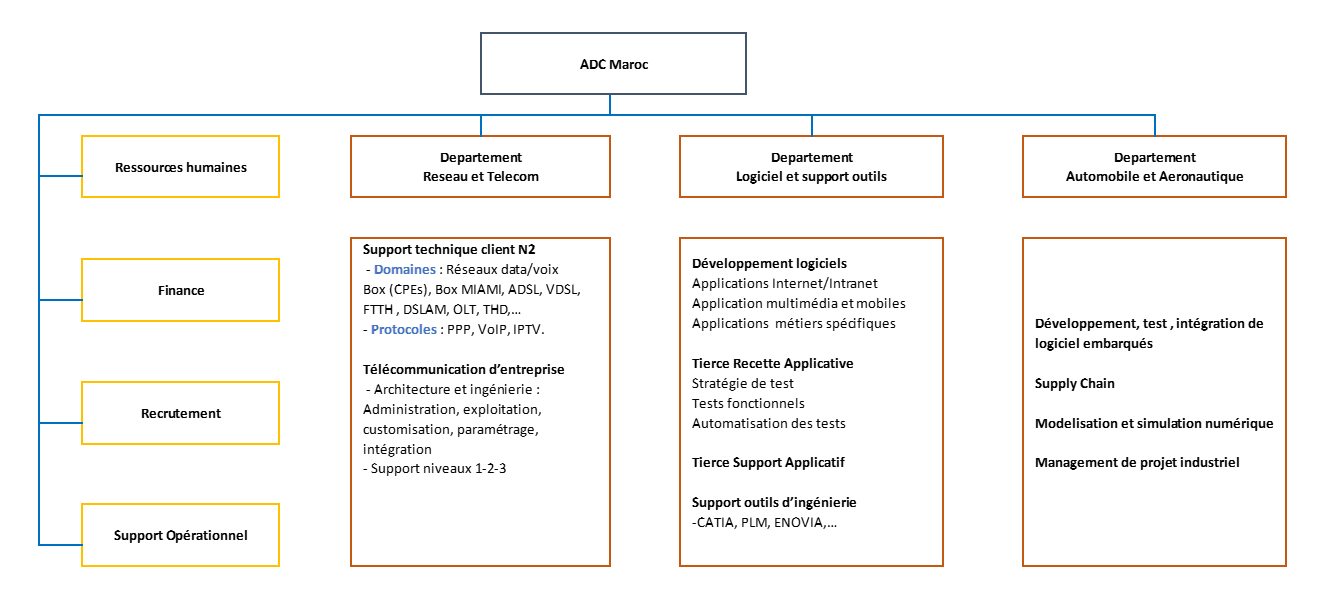
\includegraphics[scale=0.45]{images/alten_arch}
 \caption{Structure Alten}
\end{figure}

\textbf{Département Logiciel ou Software :} Ce département intervient en conseil ou en réalisation de projets complets dans le domaine de développement logiciel et dans l’assistance applicative.

\textbf{Département Réseaux et Télécommunication :} Constitué d’environ 150 consultants, ce service a comme but de gérer le support technique pour les clients de l’opérateur Bouygues Telecom sur toutes sortes de technologies.

\textbf{Département Automobile et Aéronautique :} constituée d’environ 25 ingénieurs et représente l’équipe où on m’a intégré afin d’accomplir différentes activités et tâches professionnelles. Ce département intervient sur des projets de développement et de test des systèmes embarqués dans le domaine de l’automobile.

\begin{figure}[H]
 \centering
 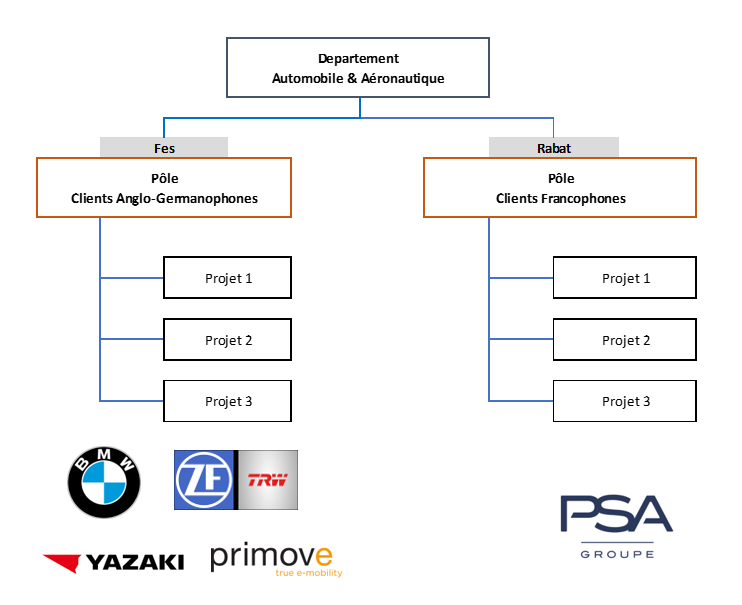
\includegraphics[scale=0.8]{images/depart_aa}
 \caption{Département Automobile et Aéronautique}
\end{figure}

En ce moment, le département Automobile du nouveau site ALTEN Rabat s’occupe principalement des projets Francophones du groupe PSA, alors que celui du Fès travaille sur des projets différents de clients Anglo-Germanophones tels que BMW, Yazaki et Primove.

\section{Présentation du projet}

Le projet où on m’a intégré me permettra de mettre en œuvre le savoir et compétences acquises durant ma formation académique, et de m’habituer à travailler dans un contexte réel du monde professionnel. Il me permettra aussi d’intégrer le milieu professionnel et de développer l’esprit d’initiative et le sens de responsabilité.

PRIMOVE, qui est la gamme électrique complète de BOMBARDIER permet aux villes et à l’industrie du transport d’intégrer facilement la mobilité électrique. Cette gamme inclut la recharge sans fil, le système de batterie compacte ainsi qu’un système de propulsion pour véhicules électriques sur rails et sur routes.

Le projet, que j’ai eu la chance d’intégrer, est le projet de recharge sans fil de PRIMOVE ou bien aussi appelé (Automatic Wireless Charging AWC). Cette technologie de recharge sans fil se base sur le principe de transfert d’énergie par induction, elle permet la transmission électrique sans contact entre les composants enfouis sous la chaussée et le récepteur installé sous le véhicule. Les composants communiquent avec le véhicules afin de s’assurer que les segments de recharge ne soient activés que lorsque le véhicule recouvre entièrement la plateforme de recharge.

\begin{figure}[H]
 \centering
 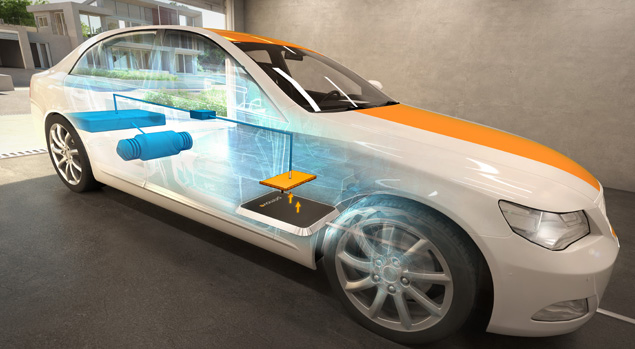
\includegraphics[scale=1.2]{images/awc_image_intro}
 \caption{Projet AWC}
\end{figure}

Le système invisible transfère l’énergie sans contact à des niveaux très hauts d’efficacité. Le système permet de charger la batterie du véhicule très rapidement. Une bobine à induction intégrée à la chaussée transporte du courant alternatif à haute fréquence, créant ainsi un champ magnétique. Ce dernier permet d’induire une tension dans le récepteur de puissance à induction du véhicule, qui est alors utilisée pour recharger et alimenter le véhicule.

Le système de recharge PRIMOVE résout les problématiques d’autonomie et de chargement, auxquels font face la mobilité électrique, avec un transfert d’énergie rapide et à haute puissance. Les postes de chargements sont installés dans des endroits stratégiques, là où les véhicules s’arrêtent le plus souvent tels que les aires de repos, les aéroports et les parkings en général.

Le système est conçu afin de respecter la sécurité et la santé des passagers, du chauffeur, des piétons ainsi que du personnel opérationnel. Les postes de recharge sont seulement allumés lorsque le véhicule est entièrement positionné au-dessus. Les champs électromagnétiques sont créés uniquement pendant la recharge et contenue entièrement sous le véhicule.

\section{Cahier des charges}

\noindent Pendant ce stage, nous étions amenés à contourner plusieurs obstacles, parmi eux : 

\begin{itemize}
	\item Compréhension du système AWC et son fonctionnement.
	\item Complexité dans l’analyse des exigences.
	\item Manque d’informations, documentation non claire.
	\item Rédaction des cas de tests.
	\item Familiarisation avec l’outil de développement de test.
	\item Difficulté d’avoir un banc de test au Maroc.
\end{itemize}


Vu que le système AWC est composé de plusieurs fonctions ou modules, ces derniers ont été distribués sur les ingénieurs travaillant sur ce projet. Pour ma part, j’étais chargé de m’occuper de la fonction « Sécurité » du système AWC, par conséquent j’avais comme objectif de : 

\begin{itemize}
	\item Créer des spécifications de tests système dans DOORS.
	\item Développer les tests cases correspondants avec EXAM.
	\item Exécuter les tests cases dans le HIL (Hardware In Loop).
	\item Analyser les rapports d’exécutions des tests cases.	
	\item Assurer la qualité de ces activités.
\end{itemize}

\section{Méthode de travail}

Le cycle en V est une méthode de gestion de projet conçue pour l’industrie. Il est une évolution du cycle en cascade qui manquait de réactivité. Il évite les retours en cas d’anomalie rencontrées. Il est composé d’une phase descendante puis montante, la phase montante envoie des informations vis-à-vis de la phase descendante.

\begin{figure}[H]
 \centering
 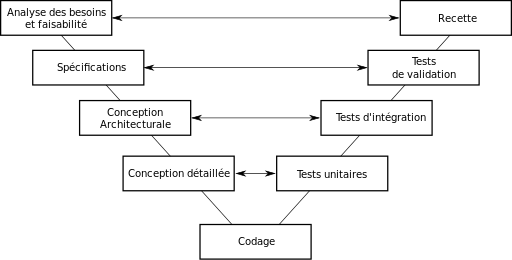
\includegraphics[scale=0.9]{images/cycle_v}
 \caption{Cycle en V}
\end{figure}

\noindent Le cycle en V est un cycle composé de 3 grandes phases contenant 8 étapes de conception d’un produit : 

\begin{itemize}
	\item La phase de conception
		\begin{itemize}
			\item Analyse des besoins et faisabilité
			\item Spécifications
			\item Conception Architecturale 
			\item Conception détaillée
		\end{itemize}
	\item La phase de réalisation
		\begin{itemize}
			\item Codage
			\item Tests unitaires
		\end{itemize}
	\item La phase de validation 
		\begin{itemize}
			\item Tests d'intégration
			\item Tests de validation
			\item Recette
		\end{itemize}
\end{itemize}

Durant la première phase \textbf{Analyse et faisabilité}, une analyse est effectuée afin de déterminer l'ensemble des fonctionnalités et les besoins du client. Ce dernier recherche un produit et il exprime ses besoins à travers ce produit. Il définit un délai final de rendu. Le prestataire effectue alors une étude de faisabilité afin de savoir si la solution peut être conçue et rentable. Le client et le prestataire définissent alors un cahier des charges détaillant toutes les fonctionnalités recherchées dans le produit final avant sa conception. Un autre composant unique et propre au cycle en V est que, lors de chaque étape de la conception, les tests correspondants sont également conçus pour être mis en œuvre plus tard au cours des phases de test.

Après le première phase, une documentation des exigences du client a été créé, celle-ci est utilisée dans la deuxième étape \textbf{Spécifications} pour générer les spécifications du systèmes qui définissent tous les composants techniques tels que les couches de données, la logique, etc. Les tests système sont également conçus au cours de cette étape.

Dans la phase \textbf{Conception Architecturale}, on précise comment le système interagit avec les différents composants soit internes soit externes. Les tests d'intégration sont également développés pendant cette période.

La phase \textbf{Conception détaillée} comprend toute la conception de bas niveau du système, et décrit comment la logique du système sera implémentée en définissant des modèles, composants, interfaces et autres. Les tests unitaires doivent également être créés pendant cette phase.


% Dans la première phase, qui est la phase de conception, le client recherche un produit et il exprime ses besoins à travers ce produit. Il définit un délai final de rendu. Le prestataire effectue une étude de faisabilité afin de savoir si la solution peut être conçue et rentable. Le client et le prestataire définissent alors un cahier des charges détaillant toutes les fonctionnalités recherchées dans le produit final avant la conception du produit final. Enfin, le prestataire détermine les spécifications techniques de la solution dans la technologie choisie, il effectue une estimation de délai pour chaque fonctionnalité à développer.

Dans la phase \textbf{Codage}, l’équipe du projet se lance dans le développement du produit sur la base des spécifications techniques. Cette phase du projet consiste à concevoir les différentes fonctionnalités du produit final dans les délais attendus. Cette période devrait durer autant de temps que nécessaire pour convertir tous les documents de conception et de spécifications générés précédemment en un système fonctionnel codé. La phase de test ne devrait commencer qu'une fois l'étape codage est complète.

%Dans la phase de réalisation, l’équipe du projet se lance dans le développement du produit sur la base des spécifications techniques. Cette phase du projet consiste à concevoir les différentes fonctionnalités du produit final dans les délais attendus. A chaque fois qu’un composant est développé il est testé afin de déterminer s’il fonctionne correctement ou pas.

Maintenant on remonte dans le cycle avec des tests inverses, en commençant par les \textbf{tests unitaires} développés pendant la phase \textit{Conception détaillée}. Idéalement, cette phase devrait éliminer la grande majorité des bugs et problèmes potentiels, et sera donc la phase de test la plus longue du projet.

Cela dit, tout comme lors des tests unitaires avec d'autres modèles de développement, les tests unitaires ne peuvent pas ou ne devraient pas couvrir tous les problèmes pouvant survenir dans le système, donc les phases de test moins granulaires doivent combler ces lacunes.

Dans la phase \textbf{Tests d'intégration}, Les tests conçus pendant la phase \textit{Conception architecturale} sont exécutés ici, garantissant que le système fonctionne avec tous les composants et intégrations tierces.

De même, dans la phase \textbf{Tests de validation} ou \textbf{Tests système}, les tests créés lors de l'étape \textit{Spécifications} sont exécutés, en se focalisant principalement sur les tests de performance et de régression. C'est là que l'équipe PRIMOVE d'ALTEN intervient.

Enfin, le \textbf{Test d'acceptation} est le processus de mise en œuvre de tous les tests créés au cours de la phase initiale des exigences et doit garantir que le système est fonctionnel dans un environnement avec des données réelles, et prêt pour le déploiement et la production.

%Et enfin dans la phase de validation, les composants sont intégrés dans la solution finales pour vérifier que l’intégration ne provoque pas d’anomalies. Le produit est ensuite testé au regard des spécifications fonctionnelles, c’est là que l’équipe d’ALTEN intervient. Au fait, il y a deux équipes une qui fait des tests systèmes et une autre qui fait des tests logiciels, je faisais partie de la première.

Le cycle en V est donc adapté aux projets restreints grâce à sa nature rigoureuse et à ses phases de conception linéaire, de réalisation et de test, il n'est pas étonnant que le cycle en V est fortement utilisé dans l'industrie automobile. Dans les situations où la longueur et la portée du projet sont bien définies, le produit final est stable, les spécifications de conception et la documentation sont claires.

Il est aussi idéal pour la gestion du temps, en effet, le cycle en V est adapté aux projets qui doivent respecter une date limite stricte et respecter des dates clés tout au long du processus. Avec des étapes assez claires que toute l'équipe peut facilement comprendre et préparer, il est relativement simple de créer une chronologie pour l'ensemble du cycle de développement. Bien évidemment, l'utilisation du cycle V ne pourra en aucun cas garantir que les jalons seront toujours atteints, mais sa nature stricte impose de respecter un calendrier assez serré.

\section{Planification du projet}

Pour la bonne gestion et déroulement du projet, on s’est mis d’accord avec le client sur plan de travail. Ce dernier nous permet de définir les travaux à réaliser, fixer des objectifs, coordonner les actions, et rendre compte de l’état d’avancement du projet.

On a pu établir un plan d’action à respecter afin de bien mener et réaliser le projet, ce plan se compose des étapes suivantes : 

\begin{itemize}
	\item Première étape : Se documenter sur le projet AWC et bien comprendre les différentes parties du système.
	\item Deuxième étape : Rédiger et développer les spécifications de tests
	\item Troisième étape : Créer les scripts de tests pour chaque spécification de test.
	\item Quatrième étape : Exécuter les scripts de test sur le HIL et les réadapter selon leurs rapports d’exécution.
\end{itemize}

\begin{figure}[H]
 \centering
 
\includegraphics[scale=0.7]{images/tbd}
 \caption{Diagramme de GANT}
\end{figure}

\section{Conclusion}
Dans ce chapitre introductif, nous avons pu présenter l’organisme d’accueil dans lequel j’ai effectué mon stage ainsi expliquer de façon brève et générale le projet sur lequel notre équipe a travaillé. Le chapitre suivant aura comme objectif d’expliquer plus en détail le système AWC ainsi que de présenter l’environnement matériel et logiciel du projet.

